\documentclass[12pt]{ociamthesis}  % default square logo 
%\documentclass[12pt,beltcrest]{ociamthesis} % use old belt crest logo
%\documentclass[12pt,shieldcrest]{ociamthesis} % use older shield crest logo

%load any additional packages
\usepackage{amssymb}
\usepackage{listings}

\usepackage{color}
 
\definecolor{codegreen}{rgb}{0,0.6,0}
\definecolor{codegray}{rgb}{0.5,0.5,0.5}
\definecolor{codepurple}{rgb}{0.58,0,0.82}
\definecolor{backcolour}{rgb}{0.95,0.95,0.92}
 
\lstdefinestyle{mystyle}{
    backgroundcolor=\color{backcolour},   
    commentstyle=\color{codegreen},
    keywordstyle=\color{magenta},
    numberstyle=\tiny\color{codegray},
    stringstyle=\color{codepurple},
    basicstyle=\footnotesize,
    breakatwhitespace=false,         
    breaklines=true,                 
    captionpos=b,                    
    keepspaces=true,                 
    numbers=left,                    
    numbersep=5pt,                  
    showspaces=false,                
    showstringspaces=false,
    showtabs=false,                  
    tabsize=2,
    language=python
}
 
\lstset{style=mystyle}
%input macros (i.e. write your own macros file called mymacros.tex 
%and uncomment the next line)
%\include{mymacros}

\title{Tugas \\[1ex]     %your thesis title,
        Kecerdasan Buatan}   %note \\[1ex] is a line break in the title

\author{Nur Hanifah Amatullah}             %your name
\college{1184086\\[5ex]
Applied Bachelor of Informatics Engineering}  %your college

%\renewcommand{\submittedtext}{change the default text here if needed}
\degree{Politeknik Pos Indonesia}     %the degree
\degreedate{Bandung 2021}         %the degree date

%end the preamble and start the document
\begin{document}

%this baselineskip gives sufficient line spacing for an examiner to easily
%markup the thesis with comments
\baselineskip=18pt plus1pt

%set the number of sectioning levels that get number and appear in the contents
\setcounter{secnumdepth}{3}
\setcounter{tocdepth}{3}


\maketitle                  % create a title page from the preamble info
\begin{dedication}
`Jika Kamu tidak dapat menahan lelahnya belajar, \\
Maka kamu harus sanggup menahan perihnya Kebodohan.'\\ 
~Imam Syafi'i~\\
\end{dedication}        % include a dedication.tex file
\begin{acknowledgements}
Assalamualaikum warahmatullahi wabarakaatuh. Segala puji bagi Allah SWT yang telah memberikan kemudahan sehingga dapat menyelesaikan laporan Tugas Chapter 1 ini, tanpa bantuan-Nya maka penulis tidak dapat menyelesaikannya dengan baik dan tepat pada waktunya. Shalawat serta salam semoga terlimpahkan kepada junjungan Nabi Muhammad SAW yang akan kita nantikan syafaatnya di yaumul qimayah nanti.

Laporan ini disusun guna memenuhi kelulusan matakuliah Pemrograman II Program Studi DIV Teknik Informatika. Proses penyeselsaian laporan ini tidak luput dari bantuan berbagai pihak. Oleh karenanya, penulis mengucapkanterima kasih kepada :
\begin{enumerate}

\item Allah SWT yang telah memberikan rahmat dan hidayah-Nya
\item Orang tua yang selalu memberikan dukungan dan motivasi dalam penyelesaian laporan
\item Bapak Rolly Awangga yang telah memberikan dukungan dan bantuan dalam penyelesaian laporan
\item Teman-teman yang saya sayangi yang selalu memberikan dukungan dan motivasinya kepada penulis

\end{enumerate}

Penulis mengharapkan kritik dan saran dari pembaca jika terdapat kesalahan dalam penyusunan laporan ini sehingga penulis dapat memperbaiki penyelesaian tugas yang selanjutnya

\begin{raggedleft}

Bandung, 16 Oktober 2019

Penulis

\end{raggedleft}
\end{acknowledgements}   % include an acknowledgements.tex file
\begin{abstract}
	Modul Praktikum ini dibuat dengan tujuan memberikan acuan, bagi mahasiswa dan dosen
	Pengajar Mata Kuliah. Pada intinya buku ini menjelaskan secara lengkap tentang Standar penilian mata kuliah programan II
	di Program Studi D4 Teknik Informatika, dan juga mengatur mekanisme, teknik penulisan, serta
	penilaiannya.Dengan demikian diharapkan semua pihak yang terlibat dalam aktivitas belajar dan mengajar
	berjalan lancar dan sesuai dengan standar.
\end{abstract}          % include the abstract

\begin{romanpages}          % start roman page numbering
\tableofcontents            % generate and include a table of contents
\listoffigures              % generate and include a list of figures
\end{romanpages}            % end roman page numbering

%now include the files of latex for each of the chapters etc
\chapter{Mengenal Kecerdasan Buatan dan Scikit-Learn}

\section{Kecerdasan Buatan}
\subsection{Definisi Kecerdasan Buatan}
\par
Kecerdasan buatan atau Artificial Intelligence merupakan kecerdasan/pengetahuan yang dimodelkan dan diajarkan ke mesin agar mesin tersebut memiliki kecerdasan yang sama seperti manusia sehingga dapat membantu pekerjaan yang umumnya dilakukan oleh manusia. Untuk memiliki kecerdasan serta mengupgrade skill dari AI nya sendiri, mesin membutuhkan data untuk menambah ilmu dan pengetahuan yang dimilikinya. Adapun proses belajar AI terdiri dari learning, reasoning, dan self-correction. Jadi tidak hanya diajari oleh manusia tetapi AI akan belajar sendiri berdasarkan pengalaman ia digunakan.
\subsection{Sejarah dan Perkembangan AI}
\par
Konsep AI sendiri sebenarnya sudah ada sejak zaman yunani kuno dan berkembang pada abad pertengahan 20. Dimulai dengan sosok John McCarthy yang disebut juga sebagai "bapak AI" merupakan seorang ilmuwan yang memiliki andil besar dalam perkembangan AI. Ia mendirikan dua buah lembaga penelitian yang bergerak di bidang AI, yaitu Stanford Artificial Intelligence Laboratory dan MIT Artificial Intelligence Laboratory. Selain itu, McCarthy juga turut mengajar di dua universitas yang memiliki nama di tingkat internasional tersebut. Disanalah, McCarthy mulai mengembangkan berbagai inovasi AI di berbagai bidang misalnya human skill, vision, listening, reasoning, dan movement of limbs. McCarthy juga menciptakan sebuah bahasa pemrograman yang disebut dengan LISP dan program yang bernama programs with common sense. Di dalam program tersebut terdapat teknologi yang berfungsi sebagai resolve atau pemecah suatu masalah.  
\par
Tahun 1959, Nathaniel Rochester dan separuh dari mahasiswanya menciptakan sebuah program yang memiliki teknologi menciptakan suatu teorema dengan menggunakan pernyataan-pernyataan yang tersedia, program ini juga disebut dengan Gheometry Theorm Prover.
\par
Perkembangan AI sempat melambat dan kembali berkembang lagi sekitar tahun 1980-an. Itu dimulai dengan penemuan sebuah sistem yang dinamakan R1 yang dapat melakukan konfigurasi pada komputer baru. Sistem ini ditemukan oleh Digital Equipment Corporation (DEC) yang selanjutnya pada tahun 1981, mereka telah menjalankan 40 sistem tersebut.
\par
Pada tahun yang sama, hampir semua perusahaan di Amerika memiliki divisi di bidang AI tersendiri sehingga sebagian besar terdapat kenaikan signifikan pada pendapatan perusahaan per-tahunnya.
\par
Untuk perkembangan AI di Indonesia sendiri sudah cukup banyak tetapi belum ada ilmuwan yang membuat teknologi sampai diakui oleh dunia. Salah satu contoh generasi muda yang melakukan inovasi dan terobosan teknologi pada bidang ini adalah Digital Native. Tidak hanya di bidang teknologi, mereka mencampurkan dan membuat sinergi antara teknologi, unsur seni, dan juga unsur alam.

\section{Machine Learning}
\subsection{Supervised Learning}
\par
Supervised Learning merupakan salah satu dari contoh aplikasi atau penerapan machine learning yang dikategorikan berdasarkan label. Yang dimaksud label disini adalah target variabel ada atau tidak data tersebut. Pada supervised learning, supervise disini dimaksud dengan label di tiap datanya. Label dimaksud dengan tag suatu data yang ditambahkan dalam machine learning.
\par
Algoritma yang digunakan pada Supervised Learning adalah :
\begin{enumerate}
    \item Klasifikasi dan Regresi
    \par Contoh cara kerja dari supervised learning adalah gambar kupu-kupu di tag "kupu-kupu" di tiap gambarnya, gambar burung di tag "burung" di tiap masing-masing imagenya. Karena ini termasuk machine learning kategori, maka mempunyai klasifikasinya sendiri misalnya (kupu-kupu, burung, dll.)
    \par
    Regresinya sendiri contoh (berat badan, tinggi badan, bentuk mata, bentuk mulut/parah, antena, dll.)
    \item Logistic Regression
    \item Model Ensemble
    \item Time Series
\end{enumerate}
\subsection{Unsupervised Learning}
\par
Unsupervised Learning memiliki beberapa keunggulan dibandingkan dengan Supervised Learning. Ia tidak menggunakan label dalam memprediksi variabel tetapi melihat kesamaan atas atribut-atribut yang dimiliki oleh variabel. Jika atribut-atribut yang diperiksa memiliki kemiripan maka akan dikelompokkan (clustering).
\par
Algoritma yang digunakan pada Unsupervised Learning adalah :
\begin{enumerate}
    \item Clustering
    \item Anomaly Detection
    \item Training Model
    \item Association Discovery
\end{enumerate}

\section{Data Set, Training Set, dan Testing Set}
\subsection{Data Set}
\par
Yang dimaksud dengan data set adalah data yang berfungsi untuk dipelajari/dilampaui oleh machine learning untuk mencapai tujuannya. Data Set ini terbagi lagi menjadi dua jenis tergantung fungsinya.
\subsection{Training Set}
\par
Merupakan data set yang digunakan untuk mencapai goal dari machine learning. Nantinya akan digunakan untuk membuat model suatu machine learning.
\subsection{Testing Set}
\par
Merupakan data set yang akan dicapai atau dilampaui, ini akan digunakan sebagai uji performa dalam model machine learning.
Membuat file main.py dan mengisinya dengan script contoh python penggunaan selenium(minimal 20 baris) yang melibatkan inputan user, kemudian mencoba untuk mengatasi error identasi.

\section{Instalasi}
\begin{enumerate}
    \item Instalasi library scikit dari anaconda, mencoba kompilasi dan uji coba ambil
contoh kode dan lihat variabel explorer
    \begin{figure}[!htbp]
    \centering
    \includegraphics[scale=0.6]{figures/1.PNG}
    \caption{\textit{Install Library Scikit}}
    \label{Figure}
    \end{figure}
    \newpage
    \item Mencoba Loading an example dataset
    \begin{figure}[!htbp]
    \centering
    \includegraphics[scale=1]{figures/Loadingdatasets/1.PNG}
    \label{Figure}
    \end{figure}
    \par
    Penjelasan : 
    \par
    Baris ke-1, loading package yang akan digunakan;
    \par
    Baris ke-2, membuat variabel bernama iris yang isinya adalah fungsi load dataset iris. Dataset ini sudah tersedia default dari sklearn, ia berisikan 3 macam spesies bunga serta ukuran sepal dan petalnya;
    \par
    Baris ke-3, pada variabel digits akan dimuat dataset digit;
    \par
    Baris ke-4, display atau menampilkan data dari var digits;
    \par
    Baris ke-5-11 merupakan output dari digits.data;
    \par
    Baris ke-12, memuat/menampilkan fungsi target dari digits yang berisikan label;
    \par
    Baris ke-13 berisi output dari digits.target;
    \par
    Baris ke-14 Setiap slot dalam array sesuai dengan piksel, dan nilai dalam slot adalah; jumlah hitam dalam pixel
    \par
    Baris ke-15-22, output dari digits.images[0]
    \newpage
    \begin{figure}[!htbp]
    \centering
    
\includegraphics[scale=0.8]{figures/Loadingdatasets/5.PNG}
    \label{Figure}
    \end{figure}
    \par
    Penjelasan :
    \par
    Baris ke-1, menampilkan seluruh keys dalam dataset iris untuk mengetahui apa saja yang berada dalam dataset tersebut; 
    \par
    Baris ke-2, Ouput yang berupa daftar dari keys atau kata kunci yang terdapat dalam dictionary
    \begin{figure}[!htbp]
    \centering
    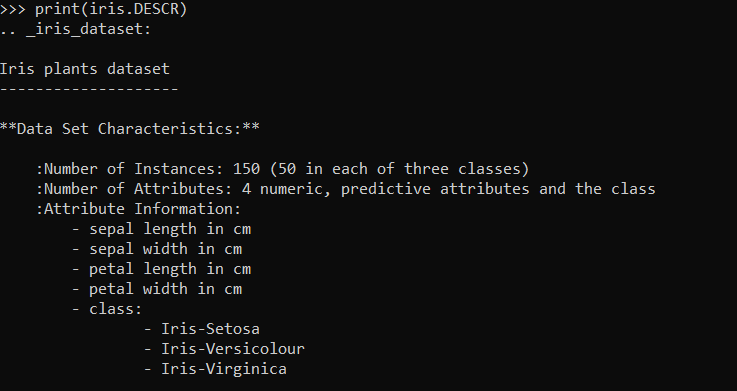
\includegraphics[scale=0.9]{figures/Loadingdatasets/6.PNG}
    \label{Figure}
    \end{figure}
    \par
    Penjelasan :
    \par
    Baris ke-1, Terdapat salah satu key DESCR pada dataset iris, dengan fungsi ini kita akan menampilkan deskripsi dari dataset;
    \par
    Baris ke-2 dst., merupakan output yang berisi deskripsi dataset iris. Dapat diketahui ia memiliki 4 atribut numerik yaitu : sepal length, sepal width, petal length, dan petal width. Selain itu ia memiliki 3 jenis spesies (class) yaitu : Iris Setosa, Iris-Versicolour, dan Iris-Virginica.
    \newpage
    \item Mencoba Learning and predicting
    \begin{figure}[!htbp]
    \centering
    \includegraphics[scale=1]{figures/Learningandpredict/1.PNG}
    \label{Figure}
    \end{figure}
    \par
    Baris ke-1, dari library sklearn import module svm (Support Vector Machine) / Algoritma Klasifikasi
    \par
    Baris ke-2, membuat variabel clf yang didalamnya memuat definisi dari fungsi SVC pada module svm yang telah diimport di awal
    \par
    Baris ke-3, menjalankan fungsi fit dari variabel clf
    \par
    Baris ke-4, output clf.fit
    \par
    Baris ke-5, menjalankan fungsi predict/prediksi dari var clf
    \par
    Baris ke-6, output clf.predict
    \item Mencoba Model persistence
    \par
    Setelah dilatih, model diharapkan untuk dapat mempertahankan model tersebut tanpa perlu dilatih kembali di masa depan. 
    \begin{figure}[!htbp]
    \centering
    \includegraphics[scale=1]{figures/Modelpersistence/1.PNG}   \label{Figure}
    \end{figure}
    \newpage
    \par
    Dalam beberapa kasus, lebih baik menggunakan joblib replacement dari pickle
    \begin{figure}[!htbp]
    \centering
    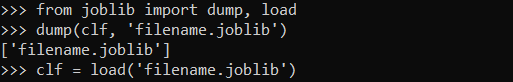
\includegraphics[scale=1]{figures/Modelpersistence/2.PNG}   \label{Figure}
    \end{figure}
    \item Mencoba Conventions
    \par
    Pada conventions sendiri, diterapkan peraturan khusus agar perilaku lebih prediktif (ketika melakukan prediksi).
    \begin{itemize}
        \item Type Casting
        \begin{figure}[!htbp]
        \centering
        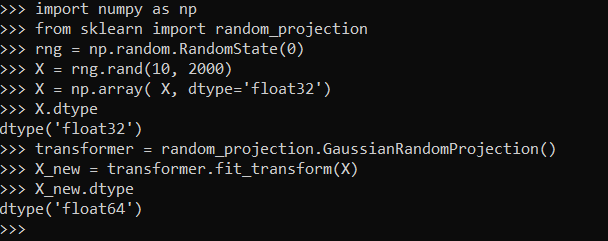
\includegraphics[scale=1]{figures/Conventions/8.PNG}
        \label{Figure}
        \end{figure}
        \item Refitting and updating parameters
        \begin{figure}[!htbp]
        \centering
        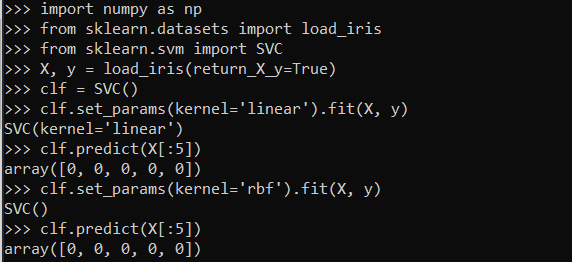
\includegraphics[scale=1]{figures/Conventions/10.PNG}
        \label{Figure}
        \end{figure}
        \newpage
        \item Multiclass vs multilabel fitting
         \begin{figure}[!htbp]
        \centering
        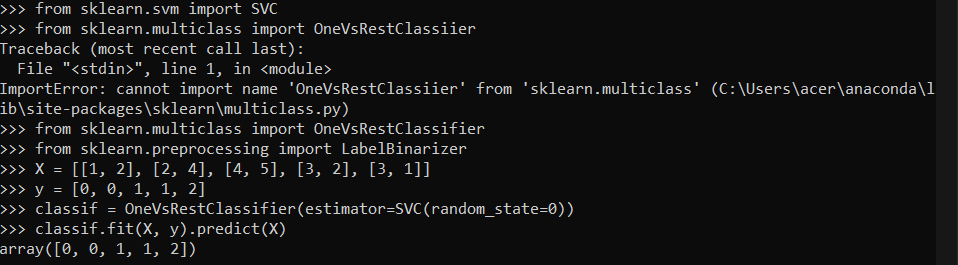
\includegraphics[scale=0.7]{figures/Conventions/11.PNG}
        \label{Figure}
        \end{figure}
        \par
        Pada kasus di atas lebih cocok untuk pengklasifikasian 1d array, sedangkan untuk 2d array :
         \begin{figure}[!htbp]
        \centering
        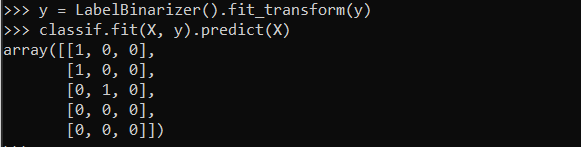
\includegraphics[scale=1]{figures/Conventions/12.PNG}
        \label{Figure}
        \end{figure}
        \par
        Pada kasus lainnya, pengklasifikasi cocok-cocok saja dengan berbagai macam contoh yang pada masing-masingnya memiliki multilable
        \begin{figure}[!htbp]
        \centering
        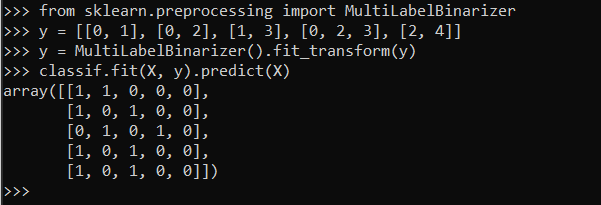
\includegraphics[scale=1]{figures/Conventions/13.PNG}
        \label{Figure}
        \end{figure}
        \par
    \end{itemize}
\end{enumerate}
\section{ Penanganan Error}
\par
Dari percobaan yang dilakukan di atas, apabila mendapatkan error maka:
\begin{enumerate}
    \item skrinsut error[hari ke 2](10)
    \item Tuliskan kode eror dan jenis errornya [hari ke 2](10)
    \item Solusi pemecahan masalah error tersebut[hari ke 2](10)
\end{enumerate}

% \chapter{Pemrograman Dasar}
Tujuan pembelajaran pada pertemuan kedua antara lain:
\begin{enumerate}
\item
Mengenal Jenis Variabel Python
\item
Input dan output user
\item
Operator Dasar
\item
Perulangan
\item
Kondisi
\item
Mengatasi Error
\item
Try Except
\end{enumerate}
Tugas dengan cara dikumpulkan dengan pull request ke github dengan menggunakan latex pada repo yang dibuat oleh asisten IRC. Kode program dipisah dalam folder src NPM.py yang berisi praktek dari masing-masing tugas file terpisah sesuai nomor yang kemudian dipanggil menggunakan input listing ke dalam file latex penjelasan atau nomor pengerjaan. Masing masing soal bernilai 5 dengan total nilai 100.

\section{Teori}
Praktek teori penunjang yang dikerjakan :
\begin{enumerate}
\item
sebutkan jenis-jenis variabel dan jelaskan cara pemakaian variabel tersebut di kode Python
\item
tuliskan bagaimana kode untuk meminta input dari user dan tuliskan bagaimana melakukan output ke layar
\item
Tuliskan operator dasar aritmatika, tambah, kali, kurang bagi, dan 
bagaimana mengubah string ke integer dan integer ke string
\item
Tuliskan dan jelaskan sintak untuk perulangan, jenis-jenisnya contoh kode dan cara pakainya di python
\item
Tuliskan jelaskan cara pakai sintak untuk memilih kondisi, dan bagiamana contoh sintak kondisi di dalam kondisi.
\item
Tuliskan apa saja jenis error yang sering ditemui di python dalam mengerjakan sintak diatas. 
dan bagaimana cara mengatasinya
\item
Tuliskan dan jelaskan cara memakai Try Except.
\end{enumerate}

\section{Ketrampilan Pemrograman}
Buat program di python dengan ketentuan:
\begin{enumerate}
\item
Buatlah luaran huruf yang dirangkai dari tanda bintang, pagar atau plus dari NPM kita.
Tanda bintang untuk NPM mod 3=0, tanda pagar untuk NPM mod 3 =1, tanda plus untuk NPM mod3=2.
Contoh Output : 
\begin{verbatim}
*****    *** ******     *****    ****
*******  *** ***  **    *** **  *****
***  ******* ******     ***  **** ***
***    ***** ***        ***       ***
***     **** ***        ***       ***
\end{verbatim}
NPM sesuai dengan nomor NPM nya.
\item
Buatlah program hello word dengan input NPM yang disimpan dalam sebuah variabel string bernama \textbf{NPM} dan output sebanyak dua dijit belakang NPM, 
contoh NPM : 113040087 maka akan ada output sebanyak 87 dengan tulisan `Hallo, 113040087 apa kabar?'
\begin{verbatim}
Input : 113040087
Output : 
Halo, 113040087 apa kabar? 
Halo, 113040087 apa kabar?
Halo, 113040087 apa kabar?
Halo, 113040087 apa kabar?
Halo, 113040087 apa kabar?
Halo, 113040087 apa kabar?
Halo, 113040087 apa kabar?
Halo, 113040087 apa kabar?
.....87 kali...
\end{verbatim}
\item
Buatlah program hello word dengan input nama yang disimpan dalam sebuah variabel string bernama \textbf{NPM} dan beri luaran output berupa tiga karakter belakang dari NPM sebanyak penjumlahan tiga dijit tersebut, 
\begin{verbatim}
Input : 113040087
Output : Halo, Nama apa kabar? 
Halo, 087 apa kabar?
Halo, 087 apa kabar?
Halo, 087 apa kabar?
Halo, 087 apa kabar?
Halo, 087 apa kabar?
Halo, 087 apa kabar?
Halo, 087 apa kabar?
........15 kali(0+8+7).........
\end{verbatim}
\item
Buatlah program hello word dengan input nama yang disimpan dalam sebuah variabel string bernama \textbf{NPM} dan beri luaran output berupa digit ketiga dari belakang dari variabel NPM, 
\begin{verbatim}
Input : 113040087
Output :
Halo, 0 apa kabar?
\end{verbatim}
\item
\label{digitvar}
(untuk soal no \ref{digitvar} dan selanjutnya wajib menggunakan perulangan dan kondisi) buat program dengan mengisi variabel alfabet dengan nomor npm satu persatu berurut.
Contoh untuk NPM : 113040087 maka,
\begin{verbatim}
a = 1
b = 1
c = 3
e = 0
f = 4
g = 0
h = 0
i = 8
j = 7
\end{verbatim}
Lakukan print NPM lengkap anda menggunakan variabel diatas :

contoh : 113040087
\item
Dari soal no \ref{digitvar}, Lakukan penjumlahan dari seluruh variabel tersebut,
\item 
Dari soal no \ref{digitvar}, Lakukan perkalian dari seluruh variabel tersebut,
\item
Dari soal no \ref{digitvar}, Lakukan print secara vertikal dari NPM anda menggunakan variabel diatas. Contoh:
\begin{verbatim}
1
1
3
0
4
0
0
8
7
\end{verbatim}
\item
Dari soal no \ref{digitvar}, Lakukan print NPM anda tapi hanya dijit genap saja. Contoh:
\begin{verbatim}
48
\end{verbatim}
\item
Dari soal no \ref{digitvar}, Lakukan print NPM anda tapi hanya dijit ganjil saja. Contoh:
\begin{verbatim}
1137
\end{verbatim}
\item 
Dari soal no \ref{digitvar}, Lakukan print NPM anda tapi hanya dijit yang termasuk bilangan prima saja. Contoh:
\begin{verbatim}
37
\end{verbatim}
\end{enumerate}


\section{Ketrampilan Penanganan Error}
Bagian Penanganan error dari script python.
\begin{enumerate}
\item
Tuliskan peringatan error yang didapat dari mengerjakan praktek kedua ini, dan jelaskan cara penanganan error tersebut.
\item
Membuat file 2err.py dan mengisinya dengan script pengisian variabel sebagai string dan pengisian variabel sebagai interger. 
Kemudian jumlahkan antara variabel integer dan string dan tangkap jenis errornya, gunakan try except untuk menunjukkan error tersebut dengan
bahasa indonesia.
\end{enumerate}


% \chapter{Fungsi dan Kelas}
Tujuan pembelajaran pada pertemuan ketiga antara lain:
\begin{enumerate}
\item
Mengenal struktur fungsi di python dalam satu file dan cara pemanggilannya
\item
Mengerti cara membuat library fungsi dan melakukan import dan berbagai jenis import
\item
Mengerti struktur library kelas python dan cara pemakaiannya
\item
Mengatasi Error yang terjadi akibat pemakaian fungsi dan kelas
\item
Try Except
\end{enumerate}
Tugas dengan cara dikumpulkan dengan pull request ke github dengan menggunakan latex pada repo yang dibuat oleh asisten IRC. Kode program dipisah dalam folder src NPM.py yang berisi praktek dari masing-masing tugas file terpisah sesuai nomor yang kemudian dipanggil menggunakan input listing ke dalam file latex penjelasan atau nomor pengerjaan. Masing masing soal bernilai 5 dengan total nilai 100. Gunakan bahasa yang baku dan bebas plagiat dengan dibuktikan hasil scan plagiarisme. Serta hasil scrinsut dari komputer sendiri, dan kode hasil sendiri.

\section{Contoh Program}
\subsection{Fungsi}
Fungsi adalah satu blok program yang terdiri dari nama fungsi, input variabel dan variabel kembalian. Nama fungsi diawali dengan \textit{def} dan setelahnya tanda titik dua. Nama bisa sama dengan isi berbeda jika menggunakan huruf besar dan kecil atau sering disebut dengan \textit{case sensitive}. Input variabel bisa lebih dari satu dengan pemisah tanda koma. variabel kembalian pasti satu, bebas apakan itu jenis \textit{string}, \textit{integer}, \textit{list} atau \textit{dictionary}. Contoh dari fungsi sederhana bisa dilihat pada listing \ref{lst:fungsisederhana}. Dimana hasil akhir variabel c adalah 15.
\begin{lstlisting}[caption=Fungsi Sederhana,label={lst:fungsisederhana}]
def Penambahan(a,b):
	r = a + b
	return r
	
	
a=2
b=13
c = Penambahan(a,b)
\end{lstlisting}
sekarang kita pisah fungsi dengan pemakaian fungsi tersebut dalam file terpisah. Kita buat file bernama \textit{kalkulator.py} yang berisi semua fungsi penambahan, pengurangan, perkalian dan pembagian seperti terlihat pada listing \ref{lst:kalkulatorlib}. Sehingga satu file yang hanya berisi semua fungsi ini kita namakan \textit{paket} atau \textit{library}.
\begin{lstlisting}[caption=Library atau Paket kalkulator,label={lst:kalkulatorlib}]
def Penambahan(a,b):
	r = a + b
	return r
def Pengurangan(a,b):
	r = a - b
	return r
def Perkalian(a,b):
	r = a * b
	return r
def Pembagian(a,b):
	r = a / b
	return r
\end{lstlisting}
	Dan satu file yang memakai fungsi tersebut dengan nama file \textit{main.py}. Karena file kalkulator.py merupakan sebuah library maka kita panggil dulu dengan menggunakan perintah \textit{import}. Harus diingat file \textit{kalkulator.py} harus satu folder dengan \textit{main.py} yang berisi seperti listing\ref{lst:pakaikalkulator}.
\begin{lstlisting}[caption=Cara penggunaan library kalkulator,label={lst:pakaikalkulator}]
import kalkulator

a=100
b=50
hasil1=kalkulator.Penambahan(a,b)
hasil2=kalkulator.Pengurangan(a,b)
hasil3=kalkulator.Perkalian(a,b)
hasil4=kalkulator.Pembagian(a,b)
\end{lstlisting}
Maka kita bisa lihat hasilnya pada variabel hasil1, hasil2, hasil3, hasil4. Pada variabel exporer di spyder.

\subsection{Kelas}
Dasarnya dari kelas adalah pemrograman berbasis objek. Maka kita harus ingat, ada kelas ada objek ada atribut ada method. Fungsi kalkulator kita ubah menjadi kelas Ngitung.py menjadi seperti pada listing \ref{lst:kelasngitung}.
\begin{lstlisting}[caption=Kelas library kalkulator,label={lst:kelasngitung}]
class Ngitung:
  def __init__(self, a, b):
    self.a = a
    self.b = b
  def Penambahan(self):
    r = self.a + self.b
    return r
  def Pengurangan(self):
    r = self.a - self.b
    return r
  def Perkalian(self):
    r = self.a * self.b
    return r
  def Pembagian(self):
    r = self.a / self.b
    return r
\end{lstlisting}
Dana pada file main.py untuk menggunakan kelas maka bedanya adalah penambahan variabel yang menjadi objek instansiasi dari kelas seperti terlihat pada listing \ref{lst:instanngitung}.
\begin{lstlisting}[caption=Cara penggunaan kelas library kalkulator,label={lst:instanngitung}]
import ngitung

a=100
b=50

hitung = ngitung.Ngitung(a,b)

hasil1=hitung.Penambahan()
hasil2=hitung.Pengurangan()
hasil3=hitung.Perkalian()
hasil4=hitung.Pembagian()
\end{lstlisting}



\section{Pemahanan Teori}
Kerjakan soal berikut ini, masing masing bernilai 5. 
Praktek teori penunjang yang dikerjakan :
\begin{enumerate}
\item
Apa itu fungsi, inputan fingsi dan kembalian fungsi dengan contoh kode program lainnya.
\item
Apa itu paket dan cara pemanggilan paket atau library dengan contoh kode program lainnya.
\item
Jelaskan Apa itu kelas, apa itu objek, apa itu atribut, apa itu method dan contoh kode program lainnya masing-masing.
\item
Jelaskan cara pemanggikan library kelas dari instansiasi dan pemakaiannya dengan contoh program lainnya.
\item
Jelaskan dengan contoh pemakaian paket dengan perintah \textit{from kalkulator import Penambahan} disertai dengan contoh kode lainnya.
\item
Jelaskan dengan contoh kodenya, pemakaian paket fungsi apabila file library ada di dalam folder.
\item
Jelaskan dengan contoh kodenya, pemakaian paket kelas apabila file library ada di dalam folder.
\end{enumerate}

\section{Ketrampilan Pemrograman}
Kerjakan soal berikut ini, masing masing bernilai 5. Pada pertemuan sebelumnya tentang pembuatan program di python, sekarang cobalah untuk membuat nya dalam bentuk fungsi dan kelas dengan ketentuan:
\begin{enumerate}
\item
Buatlah fungsi dengan inputan variabel NPM, dan melakukan print luaran huruf yang dirangkai dari tanda bintang, pagar atau plus dari NPM kita.
Tanda bintang untuk NPM mod 3=0, tanda pagar untuk NPM mod 3 =1, tanda plus untuk NPM mod3=2.
Contoh Output : 
\begin{verbatim}
*****    *** ******     *****    ****
*******  *** ***  **    *** **  *****
***  ******* ******     ***  **** ***
***    ***** ***        ***       ***
***     **** ***        ***       ***
\end{verbatim}
NPM sesuai dengan nomor NPM nya.
\item
Buatlah fungsi dengan inputan variabel berupa NPM. kemudian dengan menggunakan perulangan mengeluarkan print output sebanyak dua dijit belakang NPM, 
contoh NPM : 113040087 maka akan ada output sebanyak 87 dengan tulisan `Hallo, 113040087 apa kabar?'
\begin{verbatim}
Output : 
Halo, 113040087 apa kabar? 
Halo, 113040087 apa kabar?
Halo, 113040087 apa kabar?
Halo, 113040087 apa kabar?
Halo, 113040087 apa kabar?
Halo, 113040087 apa kabar?
Halo, 113040087 apa kabar?
Halo, 113040087 apa kabar?
.....87 kali...
\end{verbatim}
\item
Buatlah fungsi dengan dengan input variabel string bernama \textbf{NPM} dan beri luaran output dengan perulangan berupa tiga karakter belakang dari NPM sebanyak penjumlahan tiga dijit tersebut. Penjumlahan dilakukan dengan menggunakan operator aritmatika dan fungsi int() atau str().
\begin{verbatim}
Output : Halo, Nama apa kabar? 
Halo, 087 apa kabar?
Halo, 087 apa kabar?
Halo, 087 apa kabar?
Halo, 087 apa kabar?
Halo, 087 apa kabar?
Halo, 087 apa kabar?
Halo, 087 apa kabar?
........15 kali(0+8+7).........
\end{verbatim}
\item
Buatlah fungsi hello word dengan input variabel string bernama \textbf{NPM} dan beri luaran output berupa digit ketiga dari belakang dari variabel NPM menggunakan akses langsung manipulasi string pada baris ketiga dari variabel NPM.
\begin{verbatim}
Input : 113040087
Output :
Halo, 0 apa kabar?
\end{verbatim}
\item

\label{digitvar2}
(wajib menggunakan perulangan dan atau kondisi) buat fungsi program dengan input variabel NPM dan melakukan print nomor npm satu persatu kebawah.
Contoh untuk NPM : 113040087 maka,
\begin{verbatim}
1
1
3
0
4
0
0
8
7
\end{verbatim}
\item
Buatlah fungsi dengan inputan variabel NPM, didalamnya melakukan penjumlahan dari seluruh dijit NPM tersebut, wajib menggunakan perulangan dan atau kondisi.
\item 
Buatlah fungsi dengan inputan variabel NPM, didalamnya melakukan melakukan perkalian dari seluruh dijit NPM tersebut, wajib menggunakan perulangan dan atau kondisi.
\item
Buatlah fungsi dengan inputan variabel NPM, Lakukan print NPM anda tapi hanya dijit genap saja. wajib menggunakan perulangan dan atau kondisi. Contoh jika NPM :113040087.
\begin{verbatim}
48
\end{verbatim}
\item
Buatlah fungsi dengan inputan variabel NPM, Lakukan print NPM anda tapi hanya dijit ganjil saja. wajib menggunakan perulangan dan atau kondisi. Contoh jika NPM :113040087.
\begin{verbatim}
1137
\end{verbatim}
\item 
Buatlah fungsi dengan inputan variabel NPM, Lakukan print NPM anda tapi hanya dijit yang termasuk bilangan prima saja. wajib menggunakan perulangan dan atau kondisi. Contoh jika NPM :113040087.
\begin{verbatim}
37
\end{verbatim}
\item
Buatlah satu library yang berisi fungsi-fungsi dari nomor diatas dengan nama file 3lib.py dan berikan contoh cara pemanggilannya pada file main.py.
\item
Buatlah satu library class dengan nama file kelas3lib.py yang merupakan modifikasi dari fungsi-fungsi nomor diatas dan berikan contoh cara pemanggilannya  pada file main.py.
\end{enumerate}


\section{Ketrampilan Penanganan Error}
Kerjakan soal berikut ini, masing masing bernilai 5. Bagian Penanganan error dari script python.
\begin{enumerate}
\item
Tuliskan peringatan error yang didapat dari mengerjakan praktek ketiga ini, dan jelaskan cara penanganan error tersebut.
dan Buatlah satu fungsi yang menggunakan gunakan try except untuk menanggulangi error yang kemungkinan akan terjadi.
\end{enumerate}


% \chapter{Klasifikasi Teks}

Untuk pratikum saati ini menggunakan buku \textit{Python Artificial Intelligence Projects for Beginners}\cite{eckroth2018python}. Dengan praktek menggunakan python 3 dan editor anaconda dan library python scikit-learn.
Kode program ada di https://github.com/PacktPublishing/Python-Artificial-Intelligence-Projects-for-Beginners .
Tujuan pembelajaran pada pertemuan pertama antara lain:
\begin{enumerate}
\item
Mengerti implementasi klasifikasi pada teks
\item
Mengerti teknik machine learning
\item
Memahami Bag of Words
\end{enumerate}

Tugas dengan cara dikumpulkan dengan pull request ke github dengan menggunakan latex pada repo yang dibuat oleh asisten riset. Kode program menggunakan input listing ditaruh di folder src ekstensi .py dan dipanggil ke latex dengan input listings. Tulisan dan kode tidak boleh plagiat, menggunakan bahasa indonesia yang sesuai dengan gaya bahasa buku teks.

\section{Teori}
Menggunakan teknik bag-of-words pada klasifikasi berbasis text dan kata untuk mengklasifikasikan komentar yang ada di internet sebagai spam atau bukan. Atau bisa juga untuk melakukan identifikasi sebuah review apakah positive atau negatif.


\subsection{Vektorisasi data}
Pertama kita lakukan vektorisasi dari dataset. Lankah pertama kita baca terlebih dahulu dengan perintah \ref{lst:4.0}.
\begin{lstlisting}[caption=Membaca data file txt,label={lst:4.0}]
import pandas as pd
d = pd.read_csv("Youtube01-Psy.csv")
\end{lstlisting}

Memanggil library vektorisasi dari sci-kit lern, dengan menggunakan listing \ref{lst:4.1}.

\begin{lstlisting}[caption=Instansiasi Vektorizer,label={lst:4.1}]
from sklearn.feature_extraction.text import CountVectorizer
vectorizer = CountVectorizer()
\end{lstlisting}

Memilih kolom CONTENT dari dataframe d untuk di vektorisasi kemudian menampungnya pada variabel dvec menggunakan listing \ref{lst:4.2}.
\begin{lstlisting}[caption=Vektorisasi data dari atribut CONTENT,label={lst:4.2}]
dvec = vectorizer.fit_transform(d['CONTENT'])
dvec
\end{lstlisting}

Melihat daftar kata yang di vektorisasi. lalu kita simpan isinya pada variabel daptarkata dengan menggunakan perintah pada listing \ref{lst:4.3}.
\begin{lstlisting}[caption=Mendapatkan Daftar Kata,label={lst:4.3}]
daptarkata=vectorizer.get_feature_names()
\end{lstlisting}


Lakukan pengocokan data sehingga data terlihat random, perintahnya ada di listing \ref{lst:4.6}. Lalu kita cek kembali datanya pada variabel dshuf. 
\begin{lstlisting}[caption=Mengocok Data Frame,label={lst:4.6}]
dshuf = d.sample(frac=1)
\end{lstlisting}

kemudian kita melakukan pemisahan antara data set untuk training dan test dengan perintah di listing \ref{lst:4.7}.
\begin{lstlisting}[caption=Memisahkan data frame,label={lst:4.7}]
d_train=dshuf[:300]
d_test=dshuf[300:]
\end{lstlisting}

Kita lakukan training perintah listing \ref{lst:4.8}.
\begin{lstlisting}[caption=Training pada vektorisasi atau yang disebut transform dan fit,label={lst:4.8}]
d_train_att=vectorizer.fit_transform(d_train['CONTENT'])
d_train_att
\end{lstlisting}

Lalu kita lakukan transformasi saja tanpa training pada data testing dengan perintah listing \ref{lst:4.9}.
\begin{lstlisting}[caption=Transform tanpa fit dari data testing,label={lst:4.9}]
d_test_att=vectorizer.transform(d_test['CONTENT'])
d_test_att
\end{lstlisting}

Pengambilan label klasifikasi spam dari kolom CLASS dengan perintah listing \ref{lst:4.10}.
\begin{lstlisting}[caption=Pengambilan label dari data testing dan training,label={lst:4.10}]
d_train_label=d_train['CLASS']
d_test_label=d_test['CLASS']
\end{lstlisting}



\subsection{Klasifikasi dengan Random Forest}
Setelah lakukan vektorisasi. Kita panggil kelas RandomForestClassifier. dengan n estimators sebanyak 80 yang artinya kita akan membuat 80 tree dengan tanpa batasan pengambilan atribut atau kolom dengan perintah listing \ref{lst:4.11}.
\begin{lstlisting}[caption=Instansiasi kelas Random Forest,label={lst:4.11}]
from sklearn.ensemble import RandomForestClassifier
clf=RandomForestClassifier(n_estimators=80)
\end{lstlisting}


Kemudian lakukan fit untuk membangun random forest yang sudah ditentukan dengan banyak tree sebanyak 80 dengan perintah listing \ref{lst:4.12}.
\begin{lstlisting}[caption=Fitting random forest dengan dataset training,label={lst:4.12}]
clf.fit(d_train_att,d_train_label)
\end{lstlisting}


Hasilnya bisa kita lakukan prediksi dari data testing dengan perintah listing \ref{lst:4.13}.
\begin{lstlisting}[caption=Melihat Hasil prediksi,label={lst:4.13}]
clf.predict(d_test_att)
\end{lstlisting}

Untuk besaran skornya dengan perintah listing \ref{lst:4.14}
\begin{lstlisting}[caption=Score perolehan dari klasifikasi,label={lst:4.14}]
clf.score(d_test_att,d_test_label)
\end{lstlisting}

\subsection{Confusion Matrix}
Dari RF kita coba petakan ke dalam Confusion Matrix dan lihat hasilnya dengan perintah listing \ref{lst:4.15}.
\begin{lstlisting}[caption=Membuat Confusion Matrix,label={lst:4.15}]
from sklearn.metrics import confusion_matrix
pred_labels = clf.predict(d_test_att)
cm=confusion_matrix(d_test_label, pred_labels)
\end{lstlisting}



\subsection{Pengecekan Cross Validation}
Pengeceken Cross Validation untuk random forest dengan perintah \ref{lst:4.21}.
\begin{lstlisting}[caption=Hasil Cross Validation random forest,label={lst:4.21}]
from sklearn.model_selection import cross_val_score
scores = cross_val_score(clf,d_train_att,d_train_label,cv=5)

skorrata2=scores.mean()
skoresd=scores.std()
\end{lstlisting}


\section{Soal Teori}
Praktek teori penunjang yang dikerjakan(nilai 5 per nomor, untuk hari pertama) :
\begin{enumerate}
\item
Jelaskan apa itu klasifikasi teks, sertakan gambar ilustrasi buatan sendiri.
\item
Jelaskan mengapa klasifikasi bunga tidak bisa menggunakan machine learning, sertakan ilustrasi sendiri.
\item
Jelaskan bagaimana teknik pembelajaran mesin pada teks pada kata-kata yang digunakan di youtube,jelaskan arti per atribut data csv dan sertakan ilustrasi buatan sendiri.
\item
Jelaskan apa yang dimaksud vektorisasi data.
\item
Jelaskan apa itu bag of words dengan kata-kata yang sederhana dan ilustrasi sendiri.
\item
Jelaskan apa itu TF-IDF, ilustrasikan dengan gambar sendiri.
\end{enumerate}



\section{Praktek Program}
Tugas anda adalah,praktekkan dan jelaskan dengan menggunakan bahasa yang mudah dimengerti dan bebas plagiat dan wajib skrinsut dari komputer sendiri masing masing nomor di bawah ini(nilai 5 masing masing pada hari kedua).

\begin{enumerate}
\item buat aplikasi sederhana menggunakan pandas, buat data dummy format csv sebanyak 500 baris dan melakukan load ke dataframe panda.jelaskan arti setiap baris kode yang dibuat(harus beda dengan teman sekelas)
\item dari dataframe tersebut dipecah menjadi dua dataframe yaitu 450 row pertama dan 50 row sisanya(harus beda dengan teman sekelas)
\item pratekkan vektorisasi dan klasifikasi dari data (NPM mod 4, jika 0 maka katty perry, 1 LMFAO, 2 Eminem, 3 Shakira) dengan Decission Tree. Tunjukkan keluarannya dari komputer sendiri dan artikan maksud setiap luaran yang didapatkan.
\item Cobalah klasifikasikan dari data vektorisasi yang di tentukan di nomor sebelumnya dengan klasifikasi SVM. Tunjukkan keluarannya dari komputer sendiri dan artikan maksud setiap luaran yang didapatkan.
\item Cobalah klasifikasikan dari data vektorisasi yang di tentukan di nomor sebelumnya dengan klasifikasi Decission Tree. Tunjukkan keluarannya dari komputer sendiri dan artikan maksud setiap luaran yang didapatkan.
\item Plotlah confusion matrix dari praktek modul ini menggunakan matplotlib.Tunjukkan keluarannya dari komputer sendiri dan artikan maksud setiap luaran yang didapatkan.
\item jalankan program cross validaiton pada bagian teori bab ini. Tunjukkan keluarannya dari komputer sendiri dan artikan maksud setiap luaran yang didapatkan.
\item Buatlah program pengamatan komponen informasi pada bagian teori bab ini. Tunjukkan keluarannya dari komputer sendiri dan artikan maksud setiap luaran yang didapatkan.
\end{enumerate}


\section{Penanganan Error}
Dari praktek pemrograman yang dilakukan di modul ini, error yang kita dapatkan(hasil komputer sendiri) di dokumentasikan dan di selesaikan(nilai 5 per error yang ditangani. Untuk hari kedua):

\begin{enumerate}
	\item skrinsut error
	\item Tuliskan kode eror dan jenis errornya
	\item Solusi pemecahan masalah error tersebut
\end{enumerate}

\section{Presentasi Tugas}
Pada pertemuan ketiga ini, diadakan tiga penilaiain yaitu penilaian untuk tugas mingguan seperti sebelumnya dengan nilai maksimal 100. Kemudian dalam satu minggu kedepan maksimal sebelum waktu mata kuliah kecerdasan buatan. Ada presentasi kematerian dengan nilai presentasi yang terpisah masing-masing 100. Jadi ada tiga komponen penilaiain pada pertemuan ini yaitu :
\begin{enumerate}
	\item tugas minggu hari ini dan besok (maks 100). pada chapter ini
	\item presentasi Vektorisasi (maks 100). Mempraktekkan kode python dan menjelaskan cara kerjanya.
	\item presentasi cara kerja Data Frame di Pandas (maks 100).Mempraktekkan kode python dan menjelaskan cara kerjanya.
\end{enumerate}
Waktu presentasi pada jam kerja di IRC. Kriteria penilaian presentasi sangat sederhana, presenter akan ditanyai 20 pertanyaan tentang pemahamannya menggunakan python untuk kecerdasan buatan. jika presenter tidak bisa menjawab satu pertanyaan asisten maka nilai nol. Jika semua pertanyaan bisa dijawab maka nilai 100. Presentasi bisa diulang apabila gagal, sampai bisa mendapatkan nilai 100 dalam waktu satu minggu kedepan.



% \chapter{Komunikasi Perangkat Keras}

Tujuan pembelajaran pada pertemuan kelima antara lain:
\begin{enumerate}
\item
Mengenal komunikasi data serial
\item
Mengerti cara memakai library PySerial
\item
Mengerti cara instalasi driver dan menemukan BaudRate dan Nomor Port
\item
Mengatasi Error yang terjadi akibat pemakaian library csv dan pandas
\item
Try Except
\end{enumerate}
Tugas dengan cara dikumpulkan dengan pull request ke github dengan menggunakan latex pada repo yang dibuat oleh asisten IRC. Kode program dipisah dalam folder src NPM.py yang berisi praktek dari masing-masing tugas file terpisah sesuai nomor yang kemudian dipanggil menggunakan input listing ke dalam file latex penjelasan atau nomor pengerjaan. Masing masing soal bernilai 5 dengan total nilai 100. Gunakan bahasa yang baku dan bebas plagiat dengan dibuktikan hasil scan plagiarisme. Serta hasil scrinsut dari komputer sendiri, dan kode hasil sendiri. Pengerjaan menggunakan latex dan harus menyertakan file pdf hasil compile pdflatex, jika tidak diskon 50\%.


\section{Pemahaman Teori}
Kerjakan soal berikut ini, masing masing bernilai 5. Untuk hari pertama.
Praktek teori penunjang yang dikerjakan dengan deadline rabu jam 4 pagi:
\begin{enumerate}
\item
Apa itu fungsi device manager di windows dan folder /dev di linux
\item
Jelaskan langkah-langkah instalasi driver dari arduino
\item
Jelaskan bagaimana cara membaca baudrate dan port dari komputer yang sudah terinstall driver
\item
Jelaskan sejarah library pyserial
\item
Jelaskan fungsi-fungsi apa saja yang dipakai dari library pyserial
\item
Jelaskan kenapa butuh perulangan dalam tidak butuh perulangan dalam membaca serial
\item
Jelaskan bagaimana cara membuat fungsi yang mengunakan pyserial
\end{enumerate}

\section{Ketrampilan Pemrograman}
Kerjakan soal berikut ini, masing masing bernilai 10 untuk hari kamis jam 4 pagi. Soalnya adalah:

\begin{enumerate}
\item
Buatlah fungsi (file terpisah/library dengan nama NPM\_realtime.py) untuk mendapatkan data langsung dari arduino
\item
Buatlah fungsi (file terpisah/library dengan nama NPM\_save.py) untuk mendapatkan data langsung dari arduino dengan looping
\item
Buatlah fungsi (file terpisah/library dengan nama NPM\_realtime.py) untuk mendapatkan data dari arduino dan langsung ditulis kedalam file csv
\item
Buatlah fungsi (file terpisah/library dengan nama NPM\_csv.py) untuk membaca file csv hasil arduino dan mengembalikan ke fungsi
\end{enumerate}




\section{Ketrampilan Penanganan Error}
Kerjakan soal berikut ini, masing masing bernilai 5(hari kedua). Bagian Penanganan error dari script python.
\begin{enumerate}
\item
Tuliskan peringatan error yang didapat dari mengerjakan praktek ketiga ini, dan jelaskan cara penanganan error tersebut.
dan Buatlah satu fungsi yang menggunakan gunakan try except untuk menanggulangi error tersebut.
\end{enumerate}



\section{Presentasi Tugas}
Pada pertemuan ini, diadakan dua penilaiain yaitu penilaian untuk tugas mingguan seperti sebelumnya dengan nilai maksimal 100. Kemudian dalam satu minggu kedepan maksimal sebelum waktu mata kuliah pemrograman 3. Ada presentasi kematerian dengan nilai presentasi yang terpisah masing-masing 100. Jadi ada tiga komponen penilaiain pada pertemuan ini yaitu :
\begin{enumerate}
	\item tugas minggu hari ini dan besok (maks 100). pada chapter ini
	\item presentasi pyserial (maks 100). Mempraktekkan kode python dan menjelaskan cara kerjanya.
\end{enumerate}
Waktu presentasi pada jam kerja di IRC. Kriteria penilaian presentasi sangat sederhana, presenter akan ditanyai 20(10 pertanyaan program, 10 pertanyaan teori) pertanyaan tentang pemahamannya menggunakan python untuk kecerdasan buatan. jika presenter tidak bisa menjawab satu pertanyaan asisten maka nilai nol. Jika semua pertanyaan bisa dijawab maka nilai 100. Presentasi bisa diulang apabila gagal, sampai bisa mendapatkan nilai 100 dalam waktu satu minggu kedepan.





% \chapter{MFCC dan Neural Network}

Untuk pratikum saat ini menggunakan buku \textit{Python Artificial Intelligence Projects for Beginners}\cite{eckroth2018python}. Dengan praktek menggunakan python 3 dan editor spyder dan library python keras dan librosa.
Kode program ada di https://github.com/awangga/Python-Artificial-Intelligence-Projects-for-Beginners .
Tujuan pembelajaran pada pertemuan pertama antara lain:
\begin{enumerate}
\item
Mengerti konsep dasar MFCC untuk vektorisasi suara
\item
Mengerti teknik Neural Network dari hasil MFCC
\item
Memahami konsep pembobotan dan fungsi aktifasi
\end{enumerate}

Tugas dengan cara dikumpulkan dengan pull request ke github dengan menggunakan latex pada repo yang dibuat oleh asisten riset. Kode program menggunakan input listing ditaruh di folder src ekstensi .py dan dipanggil ke latex dengan input listings. \textbf{Tulisan dan kode tidak boleh plagiat}, menggunakan bahasa indonesia yang sesuai dengan gaya bahasa buku teks. Tidak menyertakan \textbf{pdf} kompilasi \textbf{diskon 50\%} nilainya.

\section{Teori}
Teori diambil dari buku referensi mengenai Neural Network dan MFCC dari dataset suara. Materi dan praktek bisa dilihat di youtube dosen.


\section{Soal Teori}
Praktek teori penunjang yang dikerjakan(nilai 5 per nomor, untuk hari pertama) :
\begin{enumerate}
\item
Jelaskan kenapa file suara harus di lakukan MFCC. dilengkapi dengan ilustrasi atau gambar.
\item
Jelaskan konsep dasar neural network.dilengkapi dengan ilustrasi atau gambar.
\item
Jelaskan konsep pembobotan dalam neural network.dilengkapi dengan ilustrasi atau gambar.
\item
Jelaskan konsep fungsi aktifasi dalam neural network. dilengkapi dengan ilustrasi atau gambar.
\item
Jelaskan cara membaca hasil plot dari MFCC,dilengkapi dengan ilustrasi atau gambar.
\item
Jelaskan apa itu one-hot encoding,dilengkapi dengan ilustrasi kode dan atau gambar.
\item
Jelaskan apa fungsi dari np.unique dan to\_categorical dalam kode program,dilengkapi dengan ilustrasi atau gambar.
\item
Jelaskan apa fungsi dari Sequential dalam kode program,dilengkapi dengan ilustrasi atau gambar.
\end{enumerate}



\section{Praktek Program}
Tugas anda adalah,praktekkan dan jelaskan dengan menggunakan bahasa yang mudah dimengerti dan bebas plagiat dan wajib skrinsut dari komputer sendiri masing masing nomor di bawah ini(nilai 5 masing masing pada hari kedua).

\begin{enumerate}
\item Jelaskan isi dari data GTZAN Genre Collection dan data dari freesound. Buat kode program untuk meload data tersebut untuk digunakan pada MFCC. Jelaskan arti dari setiap baris kode yang dibuat(harus beda dengan teman sekelas).

\item Jelaskan perbaris kode program dengan kata-kata dan dilengkapi ilustrasi gambar fungsi dari display\_mfcc() .

\item Jelaskan perbaris kode program dengan kata-kata dan dilengkapi ilustrasi gambar fungsi dari extract\_features\_song(). Jelaskan juga mengapa yang diambil 25.000 baris pertama?

\item Jelaskan perbaris kode program dengan kata-kata dan dilengkapi ilustrasi gambar fungsi dari generate\_features\_and\_labels().

\item Jelaskan dengan kata dan praktek kenapa penggunaan fungsi generate\_features\_and\_labels() sangat lama ketika meload dataset genre. Tunjukkan keluarannya dari komputer sendiri dan artikan maksud setiap luaran yang didapatkan.

\item Jelaskan kenapa harus dilakukan pemisahan data training dan data set sebesar 80 persen? Praktekkan dengan kode dan Tunjukkan keluarannya dari komputer sendiri dan artikan maksud setiap luaran yang didapatkan.

\item Praktekkan dan jelaskan masing-masing parameter dari fungsi Sequential().Tunjukkan keluarannya dari komputer sendiri dan artikan maksud setiap luaran yang didapatkan.

\item Praktekkan dan jelaskan masing-masing parameter dari fungsi compile().Tunjukkan keluarannya dengan fungsi summary dari komputer sendiri dan artikan maksud setiap luaran yang didapatkan.

\item Praktekkan dan jelaskan masing-masing parameter dari fungsi fit().Tunjukkan keluarannya dari komputer sendiri dan artikan maksud setiap luaran yang didapatkan.

\item Praktekkan dan jelaskan masing-masing parameter dari fungsi evaluate().Tunjukkan keluarannya dari komputer sendiri dan artikan maksud setiap luaran yang didapatkan.

\item Praktekkan dan jelaskan masing-masing parameter dari fungsi predict().Tunjukkan keluarannya dari komputer sendiri dan artikan maksud setiap luaran yang didapatkan.

\end{enumerate}


\section{Penanganan Error}
Dari praktek pemrograman yang dilakukan di modul ini, error yang kita dapatkan(hasil komputer sendiri) di dokumentasikan dan di selesaikan(nilai 5 per error yang ditangani. Untuk hari kedua):

\begin{enumerate}
	\item skrinsut error
	\item Tuliskan kode eror dan jenis errornya
	\item Solusi pemecahan masalah error tersebut
\end{enumerate}

\section{Presentasi Tugas}
Pada pertemuan ini, diadakan dua penilaiain yaitu penilaian untuk tugas mingguan seperti sebelumnya dengan nilai maksimal 100. Kemudian dalam satu minggu kedepan maksimal sebelum waktu mata kuliah kecerdasan buatan. Ada presentasi kematerian dengan nilai presentasi yang terpisah masing-masing 100. Jadi ada dua komponen penilaiain pada pertemuan ini yaitu :
\begin{enumerate}
	\item tugas minggu hari ini dan besok (maks 100). pada chapter ini
	\item presentasi tugas kode MFCC dan Neural Network (maks 100). Mempraktekkan kode python dan menjelaskan cara kerjanya.
\end{enumerate}
Waktu presentasi pada jam kerja di IRC. Kriteria penilaian presentasi sangat sederhana, presenter akan ditanyai 20(10 praktek dan 10 teori) pertanyaan tentang pemahamannya menggunakan python untuk kecerdasan buatan. jika presenter tidak bisa menjawab satu pertanyaan asisten maka nilai nol. Jika semua pertanyaan bisa dijawab maka nilai 100. Presentasi bisa diulang apabila gagal, sampai bisa mendapatkan nilai 100 dalam waktu satu minggu kedepan.



% \chapter{CNN}

Untuk pratikum saat ini menggunakan buku \textit{Python Artificial Intelligence Projects for Beginners}\cite{eckroth2018python}. Dengan praktek menggunakan python 3 dan editor spyder dan library python keras dan algoritma konvolusi.
Kode program ada di https://github.com/awangga/Python-Artificial-Intelligence-Projects-for-Beginners .
Tujuan pembelajaran pada pertemuan pertama antara lain:
\begin{enumerate}
\item
Mengerti konsep dasar Neural Network pada implementasi vektorisasi(Tokenize) di teks
\item
Mengerti teknik Konvolusi
\item
Memahami konsep deep learning
\end{enumerate}

Tugas dengan cara dikumpulkan dengan pull request ke github dengan menggunakan latex pada repo yang dibuat oleh asisten riset. Kode program menggunakan input listing ditaruh di folder src ekstensi .py dan dipanggil ke latex dengan input listings. \textbf{Tulisan dan kode tidak boleh plagiat}, menggunakan bahasa indonesia yang sesuai dengan gaya bahasa buku teks. Tidak menyertakan \textbf{pdf} kompilasi \textbf{diskon 50\%} nilainya.

\section{Teori}
Teori diambil dari buku referensi mengenai Neural Network dan deep learning dari dataset komentar di youtube dan HASYv2. Materi dan praktek bisa dilihat di youtube dosen.


\section{Soal Teori}
Praktek teori penunjang yang dikerjakan total nilai 100 sebagai nilai terpisah dari praktek pada modul ini(nilai 5 per nomor kecuali nomor terakhir 30 sisanya merupakan penanganan error, untuk hari pertama) :
\begin{enumerate}
\item
Jelaskan kenapa file teks harus di lakukan tokenizer. dilengkapi dengan ilustrasi atau gambar.
\item
Jelaskan konsep dasar K Fold Cross Validation pada dataset komentar Youtube pada kode listing \ref{lst:7.0}.dilengkapi dengan ilustrasi atau gambar.
\begin{lstlisting}[caption=K Fold Cross Validation,label={lst:7.0}]
kfold = StratifiedKFold(n_splits=5)
splits = kfold.split(d, d['CLASS'])
\end{lstlisting}

\item
Jelaskan apa maksudnya kode program \emph{for train, test in splits}.dilengkapi dengan ilustrasi atau gambar.
\item
Jelaskan apa maksudnya kode program \emph{train\_content = d['CONTENT'].iloc[train\_idx]} dan \emph{test\_content = d['CONTENT'].iloc[test\_idx]}. dilengkapi dengan ilustrasi atau gambar.
\item
Jelaskan apa maksud dari fungsi \emph{tokenizer = Tokenizer(num\_words=2000)} dan \emph{tokenizer.fit\_on\_texts(train\_content)}, dilengkapi dengan ilustrasi atau gambar.
\item
Jelaskan apa maksud dari fungsi \emph{d\_train\_inputs = tokenizer.texts\_to\_matrix(train\_content, mode='tfidf')} dan \emph{d\_test\_inputs = tokenizer.texts\_to\_matrix(test\_content, mode='tfidf')}, dilengkapi dengan ilustrasi kode dan atau gambar.
\item
Jelaskan apa maksud dari fungsi \emph{d\_train\_inputs = d\_train\_inputs/np.amax(np.absolute(d\_train\_inputs))} dan \emph{d\_test\_inputs = d\_test\_inputs/np.amax(np.absolute(d\_test\_inputs))}, dilengkapi dengan ilustrasi atau gambar.
\item
Jelaskan apa maksud fungsi dari \emph{d\_train\_outputs = np\_utils.to\_categorical(d['CLASS'].iloc[train\_idx])} dan \emph{d\_test\_outputs = np\_utils.to\_categorical(d['CLASS'].iloc[test\_idx])} dalam kode program, dilengkapi dengan ilustrasi atau gambar.
\item
Jelaskan apa maksud dari fungsi di listing \ref{lst:7.1}. Gambarkan ilustrasi Neural Network nya dari model kode tersebut.
\begin{lstlisting}[caption=Membuat model Neural Network,label={lst:7.1}]
       model = Sequential()
       model.add(Dense(512, input_shape=(2000,)))
       model.add(Activation('relu'))
       model.add(Dropout(0.5))
       model.add(Dense(2))
       model.add(Activation('softmax'))
\end{lstlisting}
\item
Jelaskan apa maksud dari fungsi di listing \ref{lst:7.2} dengan parameter tersebut.
\begin{lstlisting}[caption=Compile model,label={lst:7.2}]
	model.compile(loss='categorical_crossentropy', optimizer='adamax',
	                  metrics=['accuracy'])
\end{lstlisting}

\item
Jelaskan apa itu Deep Learning
\item
Jelaskan apa itu Deep Neural Network, dan apa bedanya dengan Deep Learning
\item
Jelaskan dengan ilustrasi gambar buatan sendiri(langkah per langkah) bagaimana perhitungan algoritma konvolusi dengan ukuran stride (NPM mod3+1) x (NPM mod3+1) yang terdapat max pooling.(nilai 30)

\end{enumerate}



\section{Praktek Program}
Tugas nilai terpisah dari teori maksimal 100. Praktekkan dan jelaskan dengan menggunakan bahasa yang mudah dimengerti dan bebas plagiat dan wajib skrinsut dari komputer sendiri masing masing nomor di bawah ini(nilai 5 masing masing pada hari kedua). Buka kode program pada repo Python-Artificial-Intelligence-Projects-for-Beginners pada github awangga. Buka folder Chapter04 file MathSymbols.py

\begin{enumerate}
\item Jelaskan kode program pada blok \# In[1]. Jelaskan arti dari setiap baris kode yang dibuat(harus beda dengan teman sekelas) dan hasil luarannya dari komputer sendiri.

\item Jelaskan kode program pada blok \# In[2]. Jelaskan arti dari setiap baris kode yang dibuat(harus beda dengan teman sekelas) dan hasil luarannya dari komputer sendiri.

\item Jelaskan kode program pada blok \# In[3]. Jelaskan arti dari setiap baris kode yang dibuat(harus beda dengan teman sekelas) dan hasil luarannya dari komputer sendiri.

\item Jelaskan kode program pada blok \# In[4]. Jelaskan arti dari setiap baris kode yang dibuat(harus beda dengan teman sekelas) dan hasil luarannya dari komputer sendiri.

\item Jelaskan kode program pada blok \# In[5]. Jelaskan arti dari setiap baris kode yang dibuat(harus beda dengan teman sekelas) dan hasil luarannya dari komputer sendiri.

\item Jelaskan kode program pada blok \# In[6]. Jelaskan arti dari setiap baris kode yang dibuat(harus beda dengan teman sekelas) dan hasil luarannya dari komputer sendiri.

\item Jelaskan kode program pada blok \# In[7]. Jelaskan arti dari setiap baris kode yang dibuat(harus beda dengan teman sekelas) dan hasil luarannya dari komputer sendiri.

\item Jelaskan kode program pada blok \# In[8]. Jelaskan arti dari setiap baris kode yang dibuat(harus beda dengan teman sekelas) dan hasil luarannya dari komputer sendiri.

\item Jelaskan kode program pada blok \# In[9]. Jelaskan arti dari setiap baris kode yang dibuat(harus beda dengan teman sekelas) dan hasil luarannya dari komputer sendiri.

\item Jelaskan kode program pada blok \# In[10]. Jelaskan arti dari setiap baris kode yang dibuat(harus beda dengan teman sekelas) dan hasil luarannya dari komputer sendiri.

\item Jelaskan kode program pada blok \# In[11]. Jelaskan arti dari setiap baris kode yang dibuat(harus beda dengan teman sekelas) dan hasil luarannya dari komputer sendiri.

\item Jelaskan kode program pada blok \# In[12]. Jelaskan arti dari setiap baris kode yang dibuat(harus beda dengan teman sekelas) dan hasil luarannya dari komputer sendiri.

\item Jelaskan kode program pada blok \# In[13]. Jelaskan arti dari setiap baris kode yang dibuat(harus beda dengan teman sekelas) dan hasil luarannya dari komputer sendiri.

\item Jelaskan kode program pada blok \# In[14]. Jelaskan arti dari setiap baris kode yang dibuat(harus beda dengan teman sekelas) dan hasil luarannya dari komputer sendiri.

\item Jelaskan kode program pada blok \# In[15]. Jelaskan arti dari setiap baris kode yang dibuat(harus beda dengan teman sekelas) dan hasil luarannya dari komputer sendiri.

\item Jelaskan kode program pada blok \# In[16]. Jelaskan arti dari setiap baris kode yang dibuat(harus beda dengan teman sekelas) dan hasil luarannya dari komputer sendiri.

\item Jelaskan kode program pada blok \# In[17]. Jelaskan arti dari setiap baris kode yang dibuat(harus beda dengan teman sekelas) dan hasil luarannya dari komputer sendiri.

\item Jelaskan kode program pada blok \# In[18]. Jelaskan arti dari setiap baris kode yang dibuat(harus beda dengan teman sekelas) dan hasil luarannya dari komputer sendiri.

\item Jelaskan kode program pada blok \# In[19]. Jelaskan arti dari setiap baris kode yang dibuat(harus beda dengan teman sekelas) dan hasil luarannya dari komputer sendiri.

\item Jelaskan kode program pada blok \# In[20]. Jelaskan arti dari setiap baris kode yang dibuat(harus beda dengan teman sekelas) dan hasil luarannya dari komputer sendiri.

\end{enumerate}


\section{Penanganan Error}
Dari praktek pemrograman yang dilakukan di modul ini, error yang kita dapatkan(hasil komputer sendiri) di dokumentasikan dan di selesaikan(nilai 5 per error yang ditangani. Untuk hari kedua):

\begin{enumerate}
	\item skrinsut error
	\item Tuliskan kode eror dan jenis errornya
	\item Solusi pemecahan masalah error tersebut
\end{enumerate}

\section{Presentasi Tugas}
Pada pertemuan ini, diadakan tiga penilaiain yaitu penilaian untuk tugas mingguan hari pertama dan hari kedua yang terpisah masing-masing dengan nilai maksimal 100. Kemudian dalam satu minggu kedepan maksimal sebelum waktu mata kuliah kecerdasan buatan. Ada presentasi kematerian dengan nilai presentasi yang terpisah dengan nilai maksimal 100. Jadi ada tiga komponen penilaiain pada pertemuan ini yaitu :
\begin{enumerate}
	\item tugas teori hari pertama(maks 100) modul ini
	\item tugas praktek hari kedua modul ini(maks 100)
	\item Presentasi tugas penjelasan CNN dan deep learning, Mempraktekkan kode python dan menjelaskan cara kerjanya(maks 100).
\end{enumerate}
Waktu presentasi pada jam kerja di IRC. Kriteria penilaian presentasi sangat sederhana, presenter akan ditanyai 20(10 praktek dan 10 teori) pertanyaan tentang pemahamannya menggunakan python untuk kecerdasan buatan dan teori konvolusi dan deep learning. jika presenter tidak bisa menjawab satu pertanyaan asisten maka nilai nol. Jika semua pertanyaan bisa dijawab maka nilai 100. Presentasi bisa diulang apabila gagal, sampai bisa mendapatkan nilai 100 dalam waktu satu minggu kedepan.



% \chapter{Discussion}
Please tell more about conclusion and how to the next work of this study.
% \chapter{Conditional Generative Adversarial Network}
Menggunakan sumber buku \cite{ahirwar2019gan}. Dengan source code yang ada di github awangga. 
https://github.com/awangga/Generative-Adversarial-Networks-Projects
Tujuan pembelajaran pada pertemuan pertama antara lain:
\begin{enumerate}
\item
Mengerti konsep Conditional Generative Adversarial Network
\item
Mengerti teknik CGAN
\item
Memahami penggunaan keras untuk cGAN
\end{enumerate}

Tugas dengan cara dikumpulkan dengan pull request ke github dengan menggunakan latex pada repo yang dibuat oleh asisten riset. Kode program menggunakan input listing ditaruh di folder src ekstensi .py dan dipanggil ke latex dengan input listings. \textbf{Tulisan dan kode tidak boleh plagiat}, menggunakan bahasa indonesia yang sesuai dengan gaya bahasa buku teks. Tidak menyertakan \textbf{pdf} kompilasi \textbf{diskon 50\%} nilainya.


\section{Soal Teori}
Teori diambil dari buku referensi \cite{ahirwar2019gan}  chapter 3.  Praktek teori penunjang yang dikerjakan total nilai 100 sebagai nilai terpisah dari praktek pada modul ini(nilai 9,09 per nomor kecuali nomor terakhir 30 sisanya merupakan penanganan error, untuk hari pertama) :
\begin{enumerate}
\item
Jelaskan dengan ilustrasi gambar sendiri apa perbedaan antara vanilla GAN dan cGAN.
\item
Jelaskan dengan ilustrasi gambar sendiri arsitektur dari Age-cGAN.
\item
Jelaskan dengan ilustrasi gambar sendiri arsitektur encoder network dari Age-cGAN.
\item
Jelaskan dengan ilustrasi gambar sendiri arsitektur generator network dari Age-cGAN.
\item
Jelaskan dengan ilustrasi gambar sendiri arsitektur discriminator network dari Age-cGAN.
\item
Jelaskan dengan ilustrasi gambar apa itu pretrained Inception-ResNet-2 Model.
\item
Jelaskan dengan ilustrasi gambar sendiri arsitektur Face recognition network Age-cGAN.
\item
Sebutkan dan jelaskan serta di sertai contoh-contoh tahapan dari Age-cGAN
\item
Berikan contoh perhitungan fungsi training objektif
\item
Berikan contoh dengan ilustrasi penjelasan dari Initial latent vector approximation
\item
Berikan contoh perhitungan latent vector optimization
\end{enumerate}


\section{Praktek Program}
Tugas nilai terpisah dari teori maksimal 100. Praktekkan dengan menjalankan kode program nya dan jelaskan (diperlihatkan di video youtube) dengan menggunakan bahasa yang mudah dimengerti dan bebas plagiat dan wajib diambil dari layar komputer sendiri masing masing nomor di bawah ini(nilai 15 masing masing pada hari kedua). Buka kode program pada repo Generative-Adversarial-Networks-Projects pada github awangga. Buka folder Chapter03. Kita praktekkan Age Conditional Generative Adversarial Networks (Age-cGAN). Dataset ada di https://drive.google.com/open?id=1NoV357ZvemE5dLCGySNTo6YNXsU8LyUs
\begin{enumerate}
\item
Jelaskan bagaimana cara ekstrak file dataset Age-cGAN menggunakan google colab
\item
Jelaskan bagaimana kode program bekerja untuk melakukan load terhadap dataset yang sudah di ekstrak, termasuk bagaimana penjelasan kode program perhitungan usia
\item
Jelaskan bagaimana kode program The Encoder Network bekerja dijelaskan dengan bahawa awam dengan ilustrasi sederhana
\item
Jelaskan bagaimana kode program The Generator Network bekerja dijelaskan dengan bahawa awam dengan ilustrasi sederhana
\item
Jelaskan bagaimana kode program The Discriminator Network bekerja dijelaskan dengan bahawa awam dengan ilustrasi sederhana
\item
Jelaskan bagaimana kode program Training cGAN bekerja dijelaskan dengan bahawa awam dengan ilustrasi sederhana
\item
Jelaskan bagaimana kode program Initial dan latent vector approximation bekerja dijelaskan dengan bahawa awam dengan ilustrasi sederhana
\end{enumerate}

\section{Penanganan Error}
Dari praktek pemrograman yang dilakukan di modul ini, error yang kita dapatkan(hasil komputer sendiri) di dokumentasikan dan di selesaikan(nilai 5 per error yang ditangani. Untuk hari kedua):

\begin{enumerate}
	\item skrinsut error
	\item Tuliskan kode eror dan jenis errornya
	\item Solusi pemecahan masalah error tersebut
\end{enumerate}
% \chapter{Discussion}
Please tell more about conclusion and how to the next work of this study.
% \chapter{Discussion}
Please tell more about conclusion and how to the next work of this study.
% \chapter{Discussion}
Please tell more about conclusion and how to the next work of this study.
% \chapter{Discussion}
Please tell more about conclusion and how to the next work of this study.
% \chapter{Discussion}
Please tell more about conclusion and how to the next work of this study.

%now enable appendix numbering format and include any appendices
% \appendix
% \chapter{Form Penilaian Jurnal}

gambar \ref{form1} dan \ref{form2} merupakan contoh bagaimana reviewer menilai jurnal kita. 
\begin{figure}[ht]
      \centerline{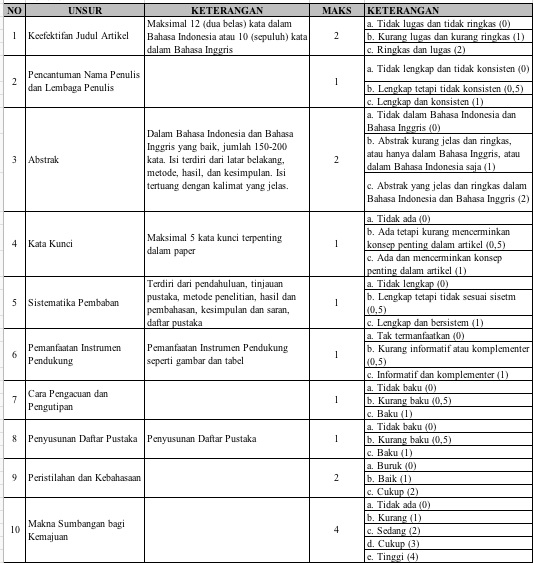
\includegraphics[width=1\textwidth]
      {figures/form1}}
      \caption{Form nilai bagian 1.}
      \label{form1}
      \end{figure}

	\begin{figure}[ht]
	      \centerline{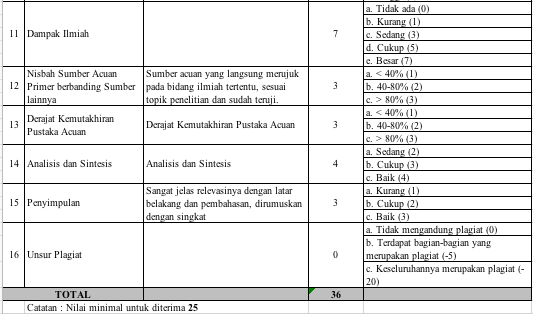
\includegraphics[width=1\textwidth]
	      {figures/form2}}
	      \caption{form nilai bagian 2.}
	      \label{form2}
	      \end{figure}

% \chapter{FAQ}

M : Kalo Intership II atau TA harus buat aplikasi ?
D : Ga harus buat aplikasi tapi harus ngoding

M : Pa saya bingung mau ngapain, saya juga bingung mau presentasi apa?
D : Makanya baca de, buka jurnal topik `ganteng' nah kamu baca dulu sehari 5 kali ya, 4 hari udah 20 tuh. Bingung itu tanda kurang wawasan alias kurang baca.

M : Pa saya sudah cari jurnal terindeks scopus tapi ga nemu.
D : Kamu punya mata de? coba dicolok dulu. Kamu udah lakuin apa aja? tolong di list laporkan ke grup Tingkat Akhir. Tinggal buka google scholar klik dari tahun 2014, cek nama jurnalnya di scimagojr.com beres.

M : Pa saya belum dapat tempat intership, jadi ga tau mau presentasi apa?
D : kamu kok ga nyambung, yang dipresentasikan itu yang kamu baca bukan yang akan kamu lakukan.

M : Pa ini jurnal harus yang terindex scopus ga bisa yang lain ?
D : Index scopus menandakan artikel tersebut dalam standar semantik yang mudah dipahami dan dibaca serta bukan artikel asal jadi. Jika diluar scopus biasanya lebih sukar untuk dibaca dan dipahami karena tidak adanya proses review yang baik dan benar terhadap artikel.

M : Pa saya tidak mengerti
D : Coba lihat standar alasan

M : Pa saya bingung
D : Coba lihat standar alasan

M : Pa saya sibuk
D : Mbahmu....

M : Pa saya ganteng
D : Ndasmu....

M : Pa saya kece
D : wes karepmu lah....


Biasanya anda memiliki alasan tertentu jika menghadapi kendala saat proses bimbingan, disini saya akan melakukan standar alasan agar persepsi yang diterima sama dan tidak salah kaprah. Penggunaan kata alasan tersebut antara lain :

1. Tidak Mengerti : anda boleh menggunakan alasan ini jika anda sudah melakukan tahapan membaca dan meresumekan 15 jurnal. Sudah mencoba dan mempraktekkan teorinya dengan mencari di youtube dan google minimal 6 jam sehari selama 3 hari berturut-turut.

2. Bingung : anda boleh mengatakan alasan bingung setelah maksimal dalam berusaha menyelesaikan tugas bimbingan dari dosen(sudah dilakukan semua). Anda belum bisa mengatakan alasan bingung jika anda masih belum menyelesaikan tugas bimbingan dan poin nomor 1 diatas. Setelah anda menyelesaikan tugas bimbingan secara maksimal dan tahap 1 poin diatas, tapi anda masih tetap bingung maka anda boleh memakai alasan ini.

%next line adds the Bibliography to the contents page
\addcontentsline{toc}{chapter}{Bibliography}
%uncomment next line to change bibliography name to references
%\renewcommand{\bibname}{References}
\bibliography{references}        %use a bibtex bibliography file refs.bib
\bibliographystyle{plain}  %use the plain bibliography style

\end{document}

